\documentclass{article}
\usepackage[margin=1in]{geometry}
\usepackage{microtype}
\usepackage{setspace}
\usepackage{amsmath}
\usepackage{parskip}
\usepackage{amssymb}
\usepackage{graphicx}

\graphicspath{{../public/}}

\parskip=4ex
\date{}
\author{}

\title{12.4 Application of Double Integrals}

\begin{document}
    \maketitle

    \textbf{Introduction}\\
    Imagine a lamina with variable density and suppouse said lamina occupies a region $ D $ of the region $ xy $ plane and its density (in units of mass per unit area) at a point $ (x,y) $ in $ D $ is given by $ Q(x,y) $, where $ Q $ is a continuous function on $ D $. This means that
    \[
        Q(x,y) = \lim \frac{\Delta m}{\Delta A} 
    \]

    where $ \Delta m ~\&~ \Delta A $ are the mass and area of a small ectangle that contains $ (x,y) $ and the limit is taken as the dimensions of the rectangle approach $ 0 $.
    
    \begin{center}
        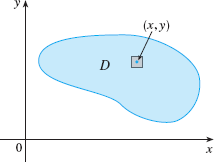
\includegraphics[width=6cm]{12_4_1}
    \end{center}

    To find the total mass $ m $ of the lamina, a rectangle $ R $ that contains $ D $ is divided into subrectangles $ R_{ij}  $ and consider $ Q(x,y) $ to be $ 0 $ outide $ D $. By choosing a point $ (x^{*}_{ij},y^{*}_{ij}) $ in $ R_{ij} $, then the mass of the part of the lamina occupying $ R_{ij} $ is approximately $ \rho(x^{*}_{ij},y^{*}_{ij}) \Delta A_{ij} $, where $ \Delta A_{ij} $ is the area of $ R_{ij} $. By adding all such masses, an approximation of the total mass is obtained.
    \[
      m \approx \sum^{k}_{i=1} \sum^{l}_{j=1} \rho(x^{*}_{ij},y^{*}_{ij}) \Delta A_{ij}  
    \]

    \begin{center}
        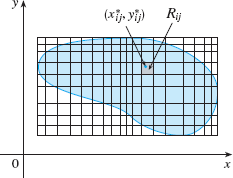
\includegraphics[width=6cm]{12_4_2}
    \end{center}

    By taking the finer partitions using smaller rectangles, the total mass $ m $ of the lamina is obtained through the limit of our summation.
    \[
      m = \lim_{\text{max } \Delta x_{i} , \Delta y_{j} \to 0}{\sum^{k}_{i=1} \sum^{l}_{j=1} \rho(x^{*}_{ij},y^{*}_{ij}) \Delta A_{ij} } = \iint_{D} \rho(x,y) ~dA 
    \]
    
   Other types of density are treated in the same manner by physicists. AN example would be an electric charge distrubuted over a region $ D $ and the charge desnity (in units of charge per unit area)is given by $ \sigma(x,y) $ at a point $ (x,y) $ in $ D $, then the total charge $ Q $ is given by
   \[
       Q = \iint_D \sigma(x,y)~dA
   \]

   \textbf{Ex 1}\\
   Charge is distributed over the triangular region $ D $ in the figure below so that the cahrge density at $ (x,y) $ is $ \rho(x,y)=xy $, measured in coulombs per square meter $ C/m^{2} $. Find the total charge.

   \begin{center}
       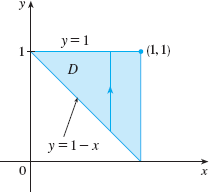
\includegraphics[width=6cm]{12_4_3}
   \end{center}

   \[
       \begin{gathered}
       Q = \iint_D \rho(x,y) ~dA = \int^{1}_{0} \int^{1}_{1-x} xy ~ dydx\\
       \int^{1}_{0} \text{\large{[}} x\frac{y^{2}}{2}  \text{\large{]}}^{y=1}_{y=1-x}~dx = \int^{1}_{0} ~ \frac{x}{2}  [1^{2}-(1-x)^{2} ]~dx\\
     \frac{1}{2} \int^{1}_{0} 2x^{2}-x^{3} ~dx=\frac{1}{2} \text{\large{[}} \frac{2x^{3}}{3}-\frac{x^{4}}{4} \text{\large{]}}^{1}_{0}=\boxed{\frac{5}{24}C}  
       \end{gathered}
   \]

  \textbf{Moments and Centers of Mass}\\
  Consider a lamina with variable density. That is suppouse the lamina occupies a region $ D $ and has density function $ \rho(x,y) $. The mass of $ R_{ij} $ is approximately $ \rho(x^{*}_{ij},y^{*}_{ij})\Delta A_{ij} $, so the moment of $ R_{ij} $ can be approximated with respect to the $ x $ axis by
  \[
    [\rho(x^{*}_{ij},y^{*}_{ij})\Delta A_{ij}]y^{*}_{ij}
  \]
  
  The moment of the entire lamina about the $ x $ axis is obtained from
  \[
    M_x = \lim_{\text{max} \Delta x_i,\Delta y_j \to 0}\sum^{m}_{i=1}\sum^{n}_{j=1}y^{*}_{ij} \rho(x^{*}_{ij},y^{*}_{ij})\Delta A_{ij} = \iint_D y\rho(x,y)~dA
  \]
  
  Similarly, the moment about the $ y $ axis is
  \[
  M_y=\lim_{\text{max}\Delta x_{i}, \Delta y_{j} \to 0} \sum^{m}_{i=1}\sum^{n}_{j=1}x^{*}_{ij}\rho(x^{*}_{ij},y^{*}_{ij})\Delta A_{ij}=\iint_D x\rho(x,y)~dA
  \]
  
  The center of mass is defined as $ (\overline{x},\overline{y}) $ so that $ m\overline{x}=M_y ~\&~ m\overline{y}=M_x $. Obtained from
  \[
    \begin{gathered}
    m=\iint_D \rho(x,y)~dA\\
    ~\\
    \overline{x}=\frac{M_y}{m}=\frac{1}{m}\iint_D x\rho(x,y)~dA \qquad \overline{y}=\frac{M_x}{m}=\frac{1}{m}\iint_D y\rho(x,y)~dA\\
    \end{gathered}
  \]

  \textbf{Ex 2}\\
  Find the mass and center of mass of a triangular lamina with verticles $ (0,0), (1,0), ~\&~ (0,2) $ if the density function is $ \rho(x,y)=1+3x+y $. The triangle's hypotenuse is calculated as $ y=2-2x $.
  \begin{center}
    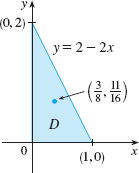
\includegraphics[width=4cm]{12_4_4}
  \end{center}

  \[
    \begin{gathered}
    m=\iint_D~dA = \int^{1}_{0} \int^{2-2x}_{0} 1+3x+y ~ dydx\\
   \int^{1}_{0} \text{\huge{[}} y+3xy+\frac{y^{2}}{2} \text{\huge{]}}^{y=2-2x}_{y=0}~dx\\
   4 \int^{1}_{0} (1-x^{2})~dx=4 \text{\huge{[}} x-\frac{x^{3}}{3} \text{\huge{]}}^{1}_0=\frac{8}{3}\\
   ~\\
   \overline{x}=\frac{1}{m}\iint_D x\rho(x,y)~dA=\frac{3}{8} \int^{1}_{0} \int^{2-2x}_{0} x+3x^{2}+xy ~ dydx\\
   \frac{3}{8} \int^{1}_{0} \text{\huge{[}} xy+3x^{2}y+x\frac{y^{2}}{2} \text{\huge{]}}^{y=2-2x}_{y=0}~dx= \frac{3}{2} \int^{1}_{0} x-x^{3}~dx\\
   \frac{3}{2} \text{\huge{[}} \frac{x^{2}}{2}-\frac{x^{4}}{4} \text{\huge{]}}^{1}_0=\frac{3}{8}\\
   ~\\
   \overline{y}=\frac{1}{m} \iint_D y\rho(x,y)~dA=\frac{3}{8} \int^{1}_{0} \int^{2-2x}_{0} y+3xy+y^{2} ~ dydx\\
   \frac{3}{8} \int^{1}_{0} \text{\huge{[}} \frac{y^{2}}{2}+3x\frac{y^{2}}{2}+\frac{y^{3}}{3} \text{\huge{]}}^{y=2-2x}_{y=0}~dx=\frac{1}{4} \int^{1}_{0} 7-9x-3x^{2}+5x^{3}~dx\\
   \frac{1}{4}\text{\huge{[}} 7x-9\frac{x^{2}}{2}-x^{3}+5\frac{x^{4}}{4} \text{\huge{]}}^{1}_{0}=\frac{11}{16}\\
   ~\\
   \boxed{(\overline{x},\overline{y})=(\frac{3}{8},\frac{11}{16})} 
    \end{gathered}
  \]

  \textbf{Ex 3}\\
  The density at any point on a semicircular lamina is proportational to the distance from the center of the circle. Find the center of mass of the lamina.

  The lamina's density at a any point on the semicircle, $ x^{2}+y^{2}=a^{2} $ is is proportional to $ K\sqrt{x^{2}+y^{2}} $. Where $ K $ is some constant and $ \sqrt{x^{2}+y^{2}} $ is the distance formula. So $ \rho(x,y)=K\sqrt{x^{2}+y^{2}} $ however we must consider the nature of the problem suggesting that we should use spherical coordiantes.

  Consider that $ \sqrt{x^{2}+y^{2}}=r  $, so $ K\sqrt{x^{2}+y^{2}}=Kr $, thus $ \rho(x,y)=Kr $.  The semicircle has a max height of $ a $ starting from $ 0 $, while it goes from $ 0 $ to $ \pi $ on the $ x $ axis. So the region $ D $ is given $ 0 \le r \le a, 0 \le \theta \le \pi $. Thus the mass of the lamina is
  \[
    \begin{gathered}
    m = \iint_D \rho(x,y)~dA= \int^{0}_{\pi} \int^{a}_{0} (Kr) r~drd\theta= \int^{\pi}_{0} \int^{a}_{0} Kr^{2} ~ drd\theta\\
    K \int^{\pi}_{0} d\theta \int^{a}_{0} r^{2} ~ dr = K\pi\frac{r^{3}}{3}\bigg|^{a}_0=\frac{K\pi a^{3}}{3} 
    \end{gathered}
  \]

  Since the lamina and density function are symmetric with respect to the $ y $ axis, so the center of mass must lie on the $ y $ axis, that is $ \overline{x}=0 $. Recall that $ y= r\sin{\theta} $ The $ y $ is given by
  \[
    \begin{gathered}
      \overline{y}= \frac{1}{m} \iint_D y\rho(x,y)~dA = \frac{3}{K\pi a^{3}} \int^{\pi}_{0} \int^{a}_{0} r\sin{\theta} (Kr)r~drd\theta\\
      \frac{3}{\pi a^{3}} \int^{\pi}_{0}\sin{\theta}~d\theta \int^{a}_{0} r^{3}~dr = \frac{3}{\pi a^{3}} \text{\huge{[}} -\cos{\theta} \text{\huge{]}}^{\pi}_0 \text{\huge{[}} \frac{r^{4}}{4} \text{\huge{]}}^{4}_0\\
      \frac{3}{\pi a^{3}} \frac{2 a^{4}}{4}= \frac{3a}{2\pi}\\
      ~\\
      \boxed{(\overline{x},\overline{y}) = (0,\frac{3a}{2\pi})}
    \end{gathered}
  \]

  \textbf{Moment of Inertia}\\
  The moment of inertia also known as the moment of a particle of mass $ m $ about an axis is defined to be $ mr^{2} $, where $ r $ is the distance from the particle to the axis. This concept is extended to a lamina with density function $ \rho(x,y) $ and occupying a region $ D $. 

  The moment of inertia about the $ x $ axis
  \[
    I_x = \lim_{\text{max} \Delta x_{ij}, \Delta y_j \to 0}\sum^{m}_{i=1} \sum^{n}_{j=1} (y^{*}_{ij})^{2} \rho(x^{*}_{ij},y^{*}_{ij}) \Delta A_{ij}= \iint_D y^{2}\rho(x,y)~dA
  \]

  Similarly, the moment of inertia about the $ y $ axis is
  \[
    I_y = \lim_{\text{max} \Delta x_i, \Delta y_j \to 0}(x^{*}_{ij},y^{*}_{ij}) \Delta A_{ij} = \iint_D x^{2} \rho(x,y)~dA
  \]

  It is also of interest to consider the moment of inertia about the origin, also called the polar moment of inertia
  \[
    I_0 = \lim_{\text{max} \Delta x_{i}, \Delta y_j \to 0} \sum^{m}_{i=1} \sum^{n}_{j=1} \text{\huge{[}} (x^{*}_{ij})^{2}+(y^{*}_{ij})^{2} \text{\huge{]}} \rho(x^{*}_{ij}, y^{*}_{ij}) \Delta A_{ij}\\
    \iint_D (x^{2}+y^{2}) \rho(x,y)~dA 
  \]

  Note that $ I_0 = I_x + I_y $ 
  
  Find the moments of inertia $ I_x, I_y, ~\&~ I_0 $ of a homogeneous disk $ D $ with density $ \rho(x,y)=\rho $, center the origin, and radius $ a $

  The boundary is the circle $ x^{2} + y^{2}=a^{2} $ and in polar coordinates $ D $  is described by $ 0 \le \theta \le 2\pi, 0 \le r \le a $. Recall that $ x^{2}+y^{2}=r^{2} $ 
  \[
    \begin{gathered}
    I_0 = \iint_D (x^{2}+y^{2})\rho~dA = \rho \int^{2\pi}_{0} \int^{a}_{0} r^{2}r ~drd\theta\\
    \rho \int^{2\pi}_{0} d\theta \int^{a}_{0} r^{3} ~ dr = 2\pi \rho \text{\huge{[}} \frac{r^{4}}{4} \text{\huge{]}}^{a}_0=\frac{\pi\rho a^{4}}{2} 
    \end{gathered}
  \]

  Based on the symmetrical nature of the problem, $ I_x=I_y $ so we can say that $ I_0=I_x+I_y \to \frac{I_0}{2}=I_x=I_y=\frac{\pi\rho a^{4}}{4} $

  Notice that the mass of the disk is
  \[
    m = \text{density} \times \text{area} = \rho(\pi a^{2})
  \]

  So the moment of inertia of the disk about the origin can be written as
  \[
    I_0 = \frac{\pi\rho a^{4}}{2}=\frac{1}{2}(\rho \pi a^{2})a^{2} = \frac{1}{2}ma^{2}
  \]

  So by increasing the mass or radius of the disk, in turn the moment of inertia is increased.

  The radius of gyration of a lamina about an axis is the number $ R $ usc that
  \[
    mR^{2}=I
  \]
  
  where $ m $ is the mass of the lamina and $ I $ is the moment of inertia about the given axis. Meaning that if the mass of the lamina were to be concentrated at a distance $ R $ from the axis, then the moment of inertia of this "point mass"would be the same as the moment of inertia of the lamina.

  So
  \[
    m \overline{y}^{2}=I_x \qquad m \overline{x}^{2}=I_y
  \]

  Thus $ (\overline{x},\overline{y}) $ is the point at which the mass of the lamina can be concentrated without changing the moments of inertia with respect to the coordinate axes.
 
  \textbf{Ex 5}\\
  Find the radius of gyration about the $ x $ axis of the disk in Example 4.
  \[
    \begin{gathered}
      m=\rho \pi a^{2} \qquad m\overline{y}^{2}=I_x \to \overline{y}^{2}=\frac{I_x}{m}\\
      \overline{y}^{2}=\frac{\frac{\pi\rho a^{4}}{4}}{\rho \pi a^{2}} =\frac{a^{2}}{4}\\
      \boxed{\overline{y}=\frac{a^{2}}{2}}
    \end{gathered}
  \]

  Therefore the radius of gyration about the $ x $ axis is $ \overline{y}=\frac{1}{2}a $, half the radius of the disk.


  

  




\end{document}
